\section{Consideration of each condition in life course}
\label{sec:consideration_life_course_conditions}

\textit{TODO: For each state, the results from the individual papers are collected.
Further individual distinctions can be derived from this (for instance in B it is is to be distinguished between intimate tracking and intimate gamification).
The types of possible data collection, tracking and also sharing is to be reported for each condition in life course.}

\subsection{Condition A: Dating - Scoping out potential intimates}
\label{subsec:A}
At the beginning of a potential relationship you want to know more about the person person of our interest. Due to this, you collect data about this person. 
\subsubsection{Searching for information}
A good way the get relevant information is using a standard social network like Facebook \footnote{\url{www.facebook.com}} or using Google search. Monitoring a person on Facebook is known as Facebook stalking \cite{levy2014intimate}. To stalk another person on Facebook undiscovered, much articles has been written about \cite{sueddeutsche_fb_stalking}. With the Website stalkscan.com \footnote{\url{https://stalkscan.com}} it is possible to get all public entries from a persons Facebook profile site which is public by only one mouse click. Surley, it can only shows what is already set public, still it make it more easily to stalk another person very quickly.
Within this website as tool is also avoided to give an involuntary like by clicking through the photographs, for instance.
The Google search mentioned at first is known as \textit{google someone}. With this method is it possible to get information from every source which is findable for the search engine \cite{nolan2005hacking}. Also for this topic there are many article how to \textit{google someone}. For instance, the search on images is of high interest \footnote{\url{https://www.lifewire.com/google-people-search-3482686}}.

\begin{table*}
	%% Table captions on top in journal version
	\caption{Interrelated types of data in \acl{QR}, source from \cite{doi:10.1080/15265161.2017.1409823}}
	\label{tab:typ_of_QR}
	\scriptsize
	\begin{center}
		\begin{tabular}{|p{4cm}|p{11cm}|p{2cm}|}
			\hline
			Intimate tracking &  Collection of all (measurable) data that can arise through intimate behaviors (in a relationship), e.g. number of partners, number of sexual encounters, duration of sexual encounter, or romantic behaviors (gifts, help in the household, attention) & SexTracker \newline SexKeeper \newline Nipple \newline Lovely \newline kGoal \\
			\hline
			Intimate gamification & Use of gamelike incentives to change or improve the behavior in a romantic relationship; Playful learning to lead a successful relationship & - \\
			\hline
			Intimate surveillance & Use of technologies to monitor intimate partners & - \\
			\hline
		\end{tabular}
	\end{center}
\end{table*}
\subsubsection{Creating and providing information}
The topic in this condition A is not only searching for data about someone, but also create such data. Levy \cite{levy2014intimate} mentioned the application Lulu as a tool to create data for use in prospective relationships. The focus of this application is on campus life. The app Lulu gives young women the opportunity to review male students and friends, with which they are connected on Facebook. The review contains information in relation to humor, manners, look and style, sex and kissing. The review giving by the female users is anonymously. In the first version, each male fiend on Facebook could be reviewed in this app. But after concerns related to privacy of reviewed male Facebook users, a review can only be committed for such male user which have explicitly allowed to this.

Furthermore, such services that combine online dating with user's geographical location are well known. Tinder is a widespread location-based dating service. The app shows potential people with different interests (e.g. romantic relationship) near to the user's location or next holiday destination \footnote{\url{https://tinder.com}}. By showing the user several profiles he/she can deside to swip right for a like. If the other person does also a right swip, it is a match. Now the user can exchange messages, for instance to get a date. The princip sound easy, but isn't at all. By using these app, a huge among of intimate data is collected. 
First of all, the tinder app is connected to Facebook and Instagram, a photo-sharing social networking service, owned by Facebook itself. In order to this there is a huge commercial interest to assume. Judith Duportail demanded access to here personal data under European data protection law after four year using the tinder app. The respons was an over 800 site report containing diffrent types of data like Facebook likes, information about education, age-rank of men she was interested in, number of Facebook friends, when and were every online conversation with her matches happened, also interests and jobs, pictures, sexual preferences. The list contains a huge amount of intimate data. In her article Duportail writes, she was amazed by how much information she was voluntarily disclosing. This was also called secondary implicit disclosed information. Firms have an increasing interest in gathering personal data from user's activities \cite{taylor2009privacy}. This results in a trade-off for the user - use the system and accept privacy concerns due to the commercial interest from the provider, or abstain the service.
Nevertheless all concerns, users reveal their data very quickly, as shown in Tait et al. \cite{tait2015hello}. 
Users who tend to gain confidence quickly, therefore, also more quickly reveal more information. In addition, this study showed that higher profile activity increases the amount of information desired. 
That means, users who maintain an active profile and present activity also receive more and higher information from other user's rather than users of profiles that provide barely information. The disclosure of information is determined in part by the personality of the user and the context in general. This affects how users surround their data online and with strangers. They found out that in only 6 - 10 minutes a user can extract the full name and date of birth from a conversation. Within these information it is easy to get further data about the person via Google search and Facebook, for instance.

In Nandwani et al. \cite{10.1007/978-3-319-61542-4_32} it was examined how quickly users reported their data to strangers and, above all, which data. For the study, an automatism was developed to contact 100 Tinder users. The study was a single blind study, so users did not know at the moment that they were writing with a Chat-bot. The evaluation of the data yielded the following results: Most of the published data was personal data, for instance: full name, date of birth, phone numbers, work details, email-addresses, complete address and other data that will not be listed here.

Why are this data disclosed to strangers in online platforms and apps? As mentioned above, the user trusts in the authenticity of the other within an active profile account. Also they do not reflect the impacts of disclosure the personal and also intimate data. For this purpose, Nandwani et al. \cite{10.1007/978-3-319-61542-4_32} suggest an virtual assistant in such applications like Tinder, which study the relationship between the users by parameters and inform the user which information should be reveal in the conversation.

\subsection{B: Tracking intimate and romantic practices}
\label{subsec:B}
The potential of creating, collecting and tracking intimate data rises if the romantic relationship between two individual goes deeper. A romantic relationship in which intimate data were tracked is named a \ac{QR}.
Danaher et al. \cite{doi:10.1080/15265161.2017.1409823} describing in their work three categories of intimate data which can be tracked in a \acs{QR}. In table \ref{tab:typ_of_QR} the three categories are summarized with a descriptions and examples.

In the following the categories intimate tracking and intimate gamification are considered in more detail.
The third category intimate surveillance will be discussed in section \ref{subsec:D}.

\subsubsection{Intimate tracking}
For the tracking of intimate data, there are a variety of apps that can be used for it.
The apps usually track the following data about sex life: \cite{doi:10.1080/15265161.2017.1409823}: 
\begin{itemize}
	\item number of partners
	\item number of "sessions" per partner
	\item sexual positions used during theses sessions
	\item number of thrusts per session
	\item duration of these sessions
	\item number of calories burned per session 
\end{itemize}
This list only mentions the most common. There are many more variants of intimate data that can be tracked. As Kelly \cite{kelly2017inevitable} mentions, nearly everything is tracked that is possible. That may not cover the big crowd, but that's also practiced.

The data is voluntarily and automatically tracked using such technology \cite{doi:10.1080/15265161.2017.1409823}. That means, the data is either actively provided by users or automatically recorded, e.g. by running the app in the background and recording audio recordings.
This type of tracking or communication is also referred to as \textit{participatory surveillance}. As Lupton \cite{doi:10.1080/13691058.2014.920528} writes, this includes looking at oneself, but for one's own purpose. Self-tracking is often associated with self-reflection, but it has less to do with it \cite{lupton2016quantified}. Rather, it is a visualization and reflection of the collected numbers. But the reflection of the self in this context involves much more than the visualization of the numerical data. This is more of a strict focus on the pure numbers. These numbers are only objectively perceived, and no longer associated with the subjective activity or context to which they once belonged.
Often, these apps also contain elements for the gamification of the mission or goals.

\subsubsection{Intimate gamification}
Another observation is the gamification in this area of tracking. Users are encouraged to quantify their sex lives in order to measure their performance and compare themselves with other users \cite{doi:10.1080/13691058.2014.920528}. This type of quantification mainly focuses on the male user.

One consequence of using such technologies may be the reinforcement of gender stereotypes \cite{doi:10.1080/13691058.2014.920528}. The algorithm defines the goals that users use to orient and measure themselves against. The individuality is lost.

In addition, this type of feedback does not necessarily have to be of good quality or have a lasting effect on relationship life. \cite{doi:10.1080/15265161.2017.1409823}. After all, a good relationship is not measured by how much sex you have or how long it lasts. As explained in the section \ref{sec:terms_of_definition} above, there are many more components that make a good relationship.

\subsubsection{Objections}
The automatic recording of such data in an app can be very questionable, because the danger is great that the user is not aware of it. Most users do not read the small print conditions of these services before using them \cite{levy2014intimate}.

Also, the sole quantification of a relationship does not necessarily lead to an improvement of the relationship skills. Rather, these types of behavioral change supports gender stereotypical reinforcement. That would be a very retrograde development compared to the current perception of our conception of love and sexuality. %TODO: Quelle für diese Behauptung suchen
In addition, as already mentioned above, the users perceive the data objectively only by quantifying the activities, similar to a sport activity like running. The reflection of the real activity is lost.

Users share this data with like-minded users, keep it for themselves and do not share it, or share it with their intimate partner.
The mere possibility of sharing this data brings with it a significantly larger audience \cite{doi:10.1080/13691058.2014.920528}. This also influences the willingness to disclose intimate data to strangers.
Users also share the data for the purpose of comparison with other users. The gamification which is often used in such apps also supports this in addition.

\subsection{C: Monitoring Fertility}
This section will focus on tracking the cycle and fertility of female users. These types of data are therefore very intimate. So far, they have been collected only in conjunction with a medical treatment and evaluated with the doctor.

The cycle and thus the connected fertility of the woman has been "monitored" for a long time. The exact beginning is unknown, it has been writing about it since the 1920s in scientific medical \cite{rotzer1988geschichte}. %TODO: Prüfen
With Josef Roetzer the symptothermal method became well known \cite{roetzer1968erweiterte}. With this method the cycle could be monitored and the fertile days could be determined exactly with a few differences.

In the age of digitization, there are of course digital technologies that support the female user to monitor the data.

In der folgenden Tabelle sind einige (bekannte) App aufgelistet.

\begin{table}
	%% Table captions on top in journal version
	\caption{App for tracking the cycle}
	\label{tab:typ_of_QR}
	\scriptsize
	\begin{center}
		\begin{tabular}{|p{1.5cm}|p{1cm}|p{4.5cm}|}
			\hline
			Bezeichnung & BS & Beschschreibung \\
			\hline
			\hline
			myNFP &  iOS \newline Android &  myNFP wertet den Zyklus nach der symptothermalen Methode (NFP) aus. Alle wichtigen Parameter für die Auswertung werden von der Nutzerin selbst eingetragen.
			\\
			\hline
			Kindara Fertility \& Ovulation  & iOS \newline Android & is based on the Fertility Awareness Method; supports the Sympto-Thermal method and can be used for Natural Family Planning (NFP) \\
			\hline
			Lily & iOS & es wird regelkonform nach symptothermaler Methode ausgewertet oder anhand von Durchschnittswerten anderer User; möchte man die App im vollen Funktionsumfang nutzen, wird ein Beitrag erhoben; dafür garantiert der Hersteller, dass die Daten nicht durch Dritte ausgewertet werden, dass die personenebzogenen Informationen nicht gespeichert werden udn auf keinem Server ein Backup der personenbezogenen Daten liegen \footnote{\url{http://whimsicallily.com/lily/en/privacypolicy.php}} \\
			\hline
			Glow & iOS \newline Android & \\
			\hline
		\end{tabular}
	\end{center}
\end{table}
Laut dem Hersteller myNFP werden die sensibeln Daten nicht durch Dritte verarbeitet. Weiterhin werden sowenig Daten erfasst wie möglich. Die Daten sind anonym und lassen nicht auf die Person zurückschließen. Der Herstellter begründet das mit dem Agrument, dass die App pro Monat  2,50 \euro{} \footnote{\url{https://www.mynfp.de/datenschutz}}.

ZUr Kindara App finden sich ebenfalls Angaben zum Datenschutz, diese sehen allerdings anders aus als in der vorhergehenden App \footnote{\url{https://www.kindara.com/privacy-policy}}:
\begin{quote}
	Kindara collects and uses the information you provide to us when you use the Kindara Service. Information that Kindara may collect includes: name, date of birth, e-mail address, fertility-related data and other family planning and health-related information you provide. You may consider some of this information to be sensitive so you should choose carefully regarding whether and if you will use the Service.
\end{quote}
 Da die App kostenlos angeboten wird, liegt die Vermutung nahe, dass die Daten weiter verarbeitet werden. ZUr App wird ein zusätzliches Device angeboten, mit welchem die Aufwachtemperator gemessen werden kann. Das Gerät connecet sich mit der App automatisch, wenn die Temperatur gemessen wird. Die Daten werden par Bluethoot an die App übermittelt \footnote{\url{https://www.kindara.com/wink}}.

\subsection{The app Glow}
Auf die Glow app möchte ich gesondert eingehen, da sehr viele Arbeiten darüber schreiben \cite{doi:10.1080/15265161.2017.1409823}, \cite{levy2014intimate} und \cite{doi:10.1080/13691058.2014.920528}.
\begin{figure}[htb]
	\centering
	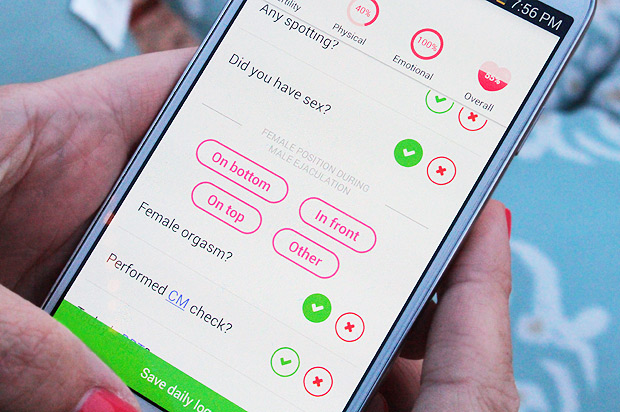
\includegraphics[width=\linewidth]{img/Glow-App-review-screenshot-1.jpg}
	\caption{Die Glow App erfasst ein Vielzahl an intimen Daten (Bildquelle: \cite{glowApp})}
	\label{fig:glow_app}
\end{figure}
Die App wurde vom PayPal founder Max Levchin in 2013 gestartet, und bietet genüber den vielen anderen Apps im Bereich Fruchtbarkeit und natürliche Verhütung eine große Konkruenz. Die Glow App trackt eine Vielzahl an Daten, unter anderen die Menstruation, position and firmness of a womens's cervix, sexual intercourse (with the women's position during ejaculation), "wheter they had an orgasm [and] wheter they experienced emotional or physical discomfort during sex" \cite{doi:10.1080/13691058.2014.920528} . Außerdem kann die Stimmung der Nutzerin getrackt werden.
Der Unterschied zu anderen Apps ist, die Glow app macht die Sammlung intimer Daten zu einer Familienangelegenheit. Die Partner der Nutzerin werden dazu eingeladen einen mirror app herunterzuladen, und zusätzliche Daten anzugeben \cite{levy2014intimate} Die App sendet dem Partner außerdem Nachrichten über den akteullen Stand der Period der Partnerin und erinnert an eine Aufmerksamkeit, wie z.B. Blumen oder eine nette Nachricht.

Die Daten der Nutzer werden gesammlet ausgewertet, um aus der großen sammlung bessere Vorhersagen für die individuellen Nutzerin angeben zu können.

Danaher et al. \cite{doi:10.1080/15265161.2017.1409823} argumentieren unter dem Punkt Gender Relationship Objection, dass diese Art der Technologien Frauen zu einem Objekt der Überwachung und Quantifizierung machen. Diese Technologien geben den Anschein, also sei der Zyklus einer Frau unüberwacht chaotisch und nur mit strenger Kontrolle "regulierbar".
ZUdem würden diese App die Entwicklung und Verstärkung von geschlechtsspezifischen Stereotypen fördern.

Die Angabe solcher intimer Daten ist zum teil sehr bedenklich, wenn die Nutzerin nicht beachtet, wie die Daten weiter ausgewertet werden. Sicherlich können diese Technologien hilfreich sein in der Auswertung der erhobenen Daten, und erinnern an die tägliche Messung. Leider werden diese sehr sensiblen Daten auch für commerziellen Zwecke genutzt. 



The first three conditions can be summarized well in the following graphic.
\begin{figure}[htb]
	\centering
	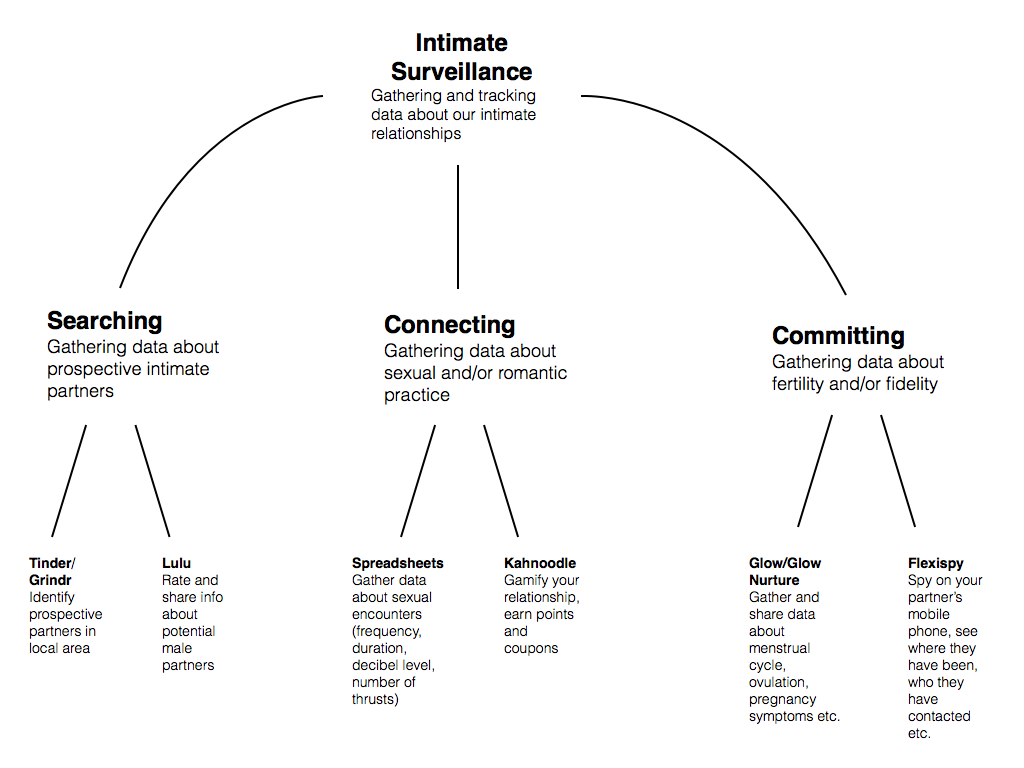
\includegraphics[width=\linewidth]{img/d372d-intimate2bsurveillance-122.png}
	\caption{Summarizing of conditions A, B and C \cite{ethicsOfSurveillance}}
	\label{fig:intimate_surveillance}
\end{figure}
\subsection{D}
"Now that mobile digital technologies that can be used for surveillance are part of everyday social life. "\cite{doi:10.1080/13691058.2014.920528}.
\label{subsec:D}
\begin{description}
	\item[A] \textit{Data collection at the beginning of a relationship, Facebook stalking, potential partner googling, Tinder. In the following: why is this used or why are these data collected, recorded etc. Subsequently, how do people perceive this, influence of data on perception}
	\item[B] \textit{Categorization in intimate tracking and intimate gamification from \acl{QR}: example of these apps and tracking devices. What added value do they have in the relationship? What's in it? How do people perceive that (Quantifying, over-trust in numbers).}
	\item[C] \textit{Drafting the role of women at this stage of a relationship: many apps and devices for tracking women (cycle, fertility, etc.).}
	\item[D] \textit{Category intimate surveillance from \acl{QR}: main emphasis:
	Tracking the partners in a relationship: acceptable or not by mutual agreement? Does that affect the relationship, or the mutual trust? There is no investigation until now (continue at the end (conclusion, further work)).}
\end{description}